\documentclass[aspectratio=169,11pt]{beamer}

\usepackage{array}
\usepackage{booktabs}
\usepackage{graphicx}
\usepackage{siunitx}
\usepackage{xcolor}

\usetheme{Madrid}
\usecolortheme{default}
\setbeamertemplate{navigation symbols}{}
\setbeamertemplate{footline}[frame number]

\definecolor{aaltoBlue}{RGB}{0,83,155}
\definecolor{goodGreen}{RGB}{35,120,75}
\definecolor{warnRed}{RGB}{170,55,55}
\definecolor{softGray}{RGB}{245,246,248}

\newcommand{\code}[1]{\texttt{\scriptsize\detokenize{#1}}}
\newcommand{\good}[1]{\textcolor{goodGreen}{#1}}
\newcommand{\warn}[1]{\textcolor{warnRed}{#1}}
\newcommand{\bluetext}[1]{\textcolor{aaltoBlue}{#1}}
\newcolumntype{L}[1]{>{\raggedright\arraybackslash}p{#1}}

\title[Mie Multi-Hole Parallel Processing]{Parallel Programming in the Multi-Hole Mie Pipeline}
\subtitle{How TB-scale top-view spray videos are reduced to plume-wise 1D metrics}
\author{Linan Jiang}
\institute{Aalto University}
\date{May 2026}

\begin{document}

\begin{frame}
  \titlepage
\end{frame}

\begin{frame}{The Runtime Result We Care About}
\small
\begin{columns}[T,onlytextwidth]
\begin{column}{0.52\linewidth}
\begin{block}{Current production-style timing}
\[
731.91~\mathrm{s} + 963.31~\mathrm{s}
= 1695.22~\mathrm{s}
\approx 28.25~\mathrm{min}.
\]
\end{block}

\vspace{0.4em}
This is for the TB-scale multi-hole Mie video archive after switching off expensive optional outputs.
\end{column}

\begin{column}{0.44\linewidth}
\begin{tabular}{L{0.58\linewidth}L{0.26\linewidth}}
\toprule
Option & Current \\
\midrule
\code{repair_bw} & \good{False} \\
\code{save_boundary_points_csv} & \good{False} \\
\code{save_preview_avi} & \good{False} \\
\code{preview_playback} & \good{False} \\
\bottomrule
\end{tabular}

\vspace{0.8em}
\footnotesize
Meaning: the timing mostly reflects the core computation, not preview videos or boundary-point file dumping.
\end{column}
\end{columns}
\end{frame}

\begin{frame}{One-Sentence Summary}
\Large
\begin{center}
The pipeline is not just a faster loop.
\end{center}

\vspace{0.6em}
\large
It is an assembly line:
\begin{itemize}
  \item \bluetext{GPU}: does the dense pixel/frame math.
  \item \bluetext{CPU threads}: compute per-plume engineering metrics.
  \item \bluetext{Background I/O}: reads the next video and writes the current results.
\end{itemize}

\vspace{0.5em}
\small
The main goal is simple: keep the expensive machine busy and avoid waiting for disk or optional visualization.
\end{frame}

\begin{frame}{The Actual Processing Pipeline}
\centering
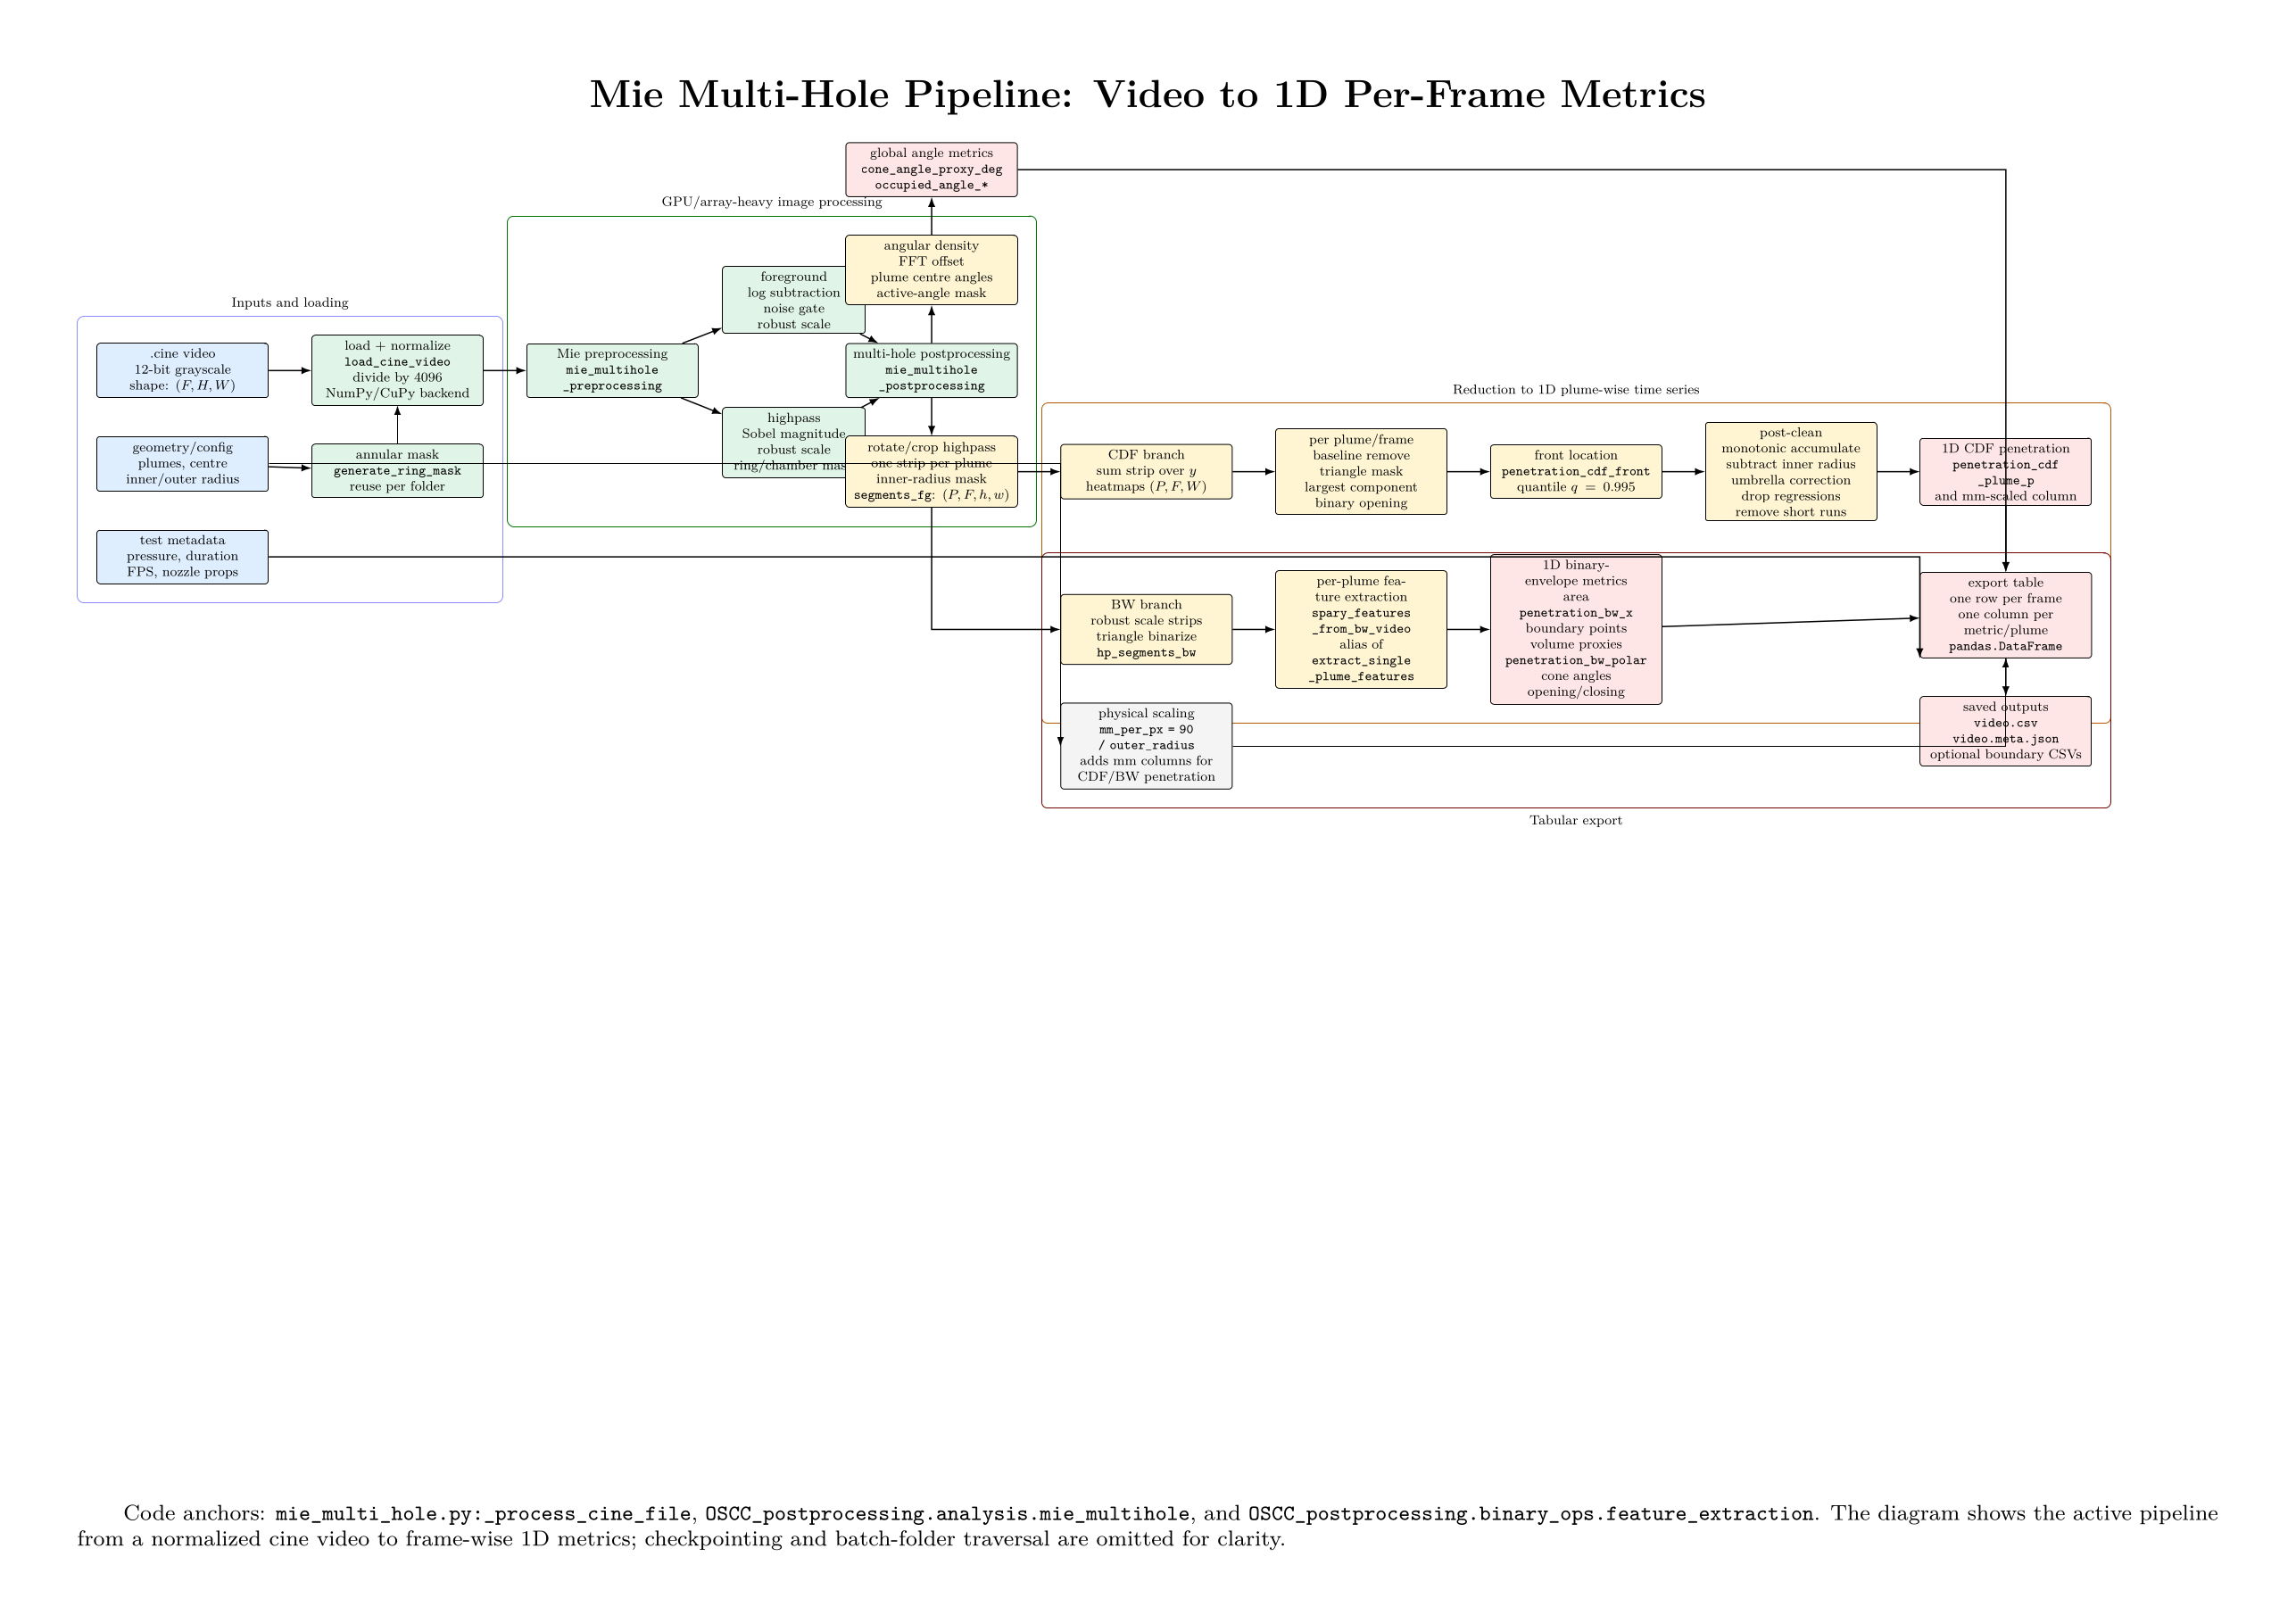
\includegraphics[
  width=0.92\linewidth,
  height=0.72\textheight,
  keepaspectratio
]{assets/mie_video_to_1d_dataflow.png}

\vspace{0.1em}
\footnotesize
The image-processing chain converts one normalized \code{.cine} video into plume-wise time series and exported CSV/metadata.
\end{frame}

\begin{frame}{Why a MATLAB-Style Loop Is Not Enough}
\small
\begin{columns}[T,onlytextwidth]
\begin{column}{0.48\linewidth}
\begin{block}{Natural MATLAB view}
\begin{enumerate}
  \item loop over videos;
  \item loop over frames;
  \item loop over pixels;
  \item loop over plumes;
  \item save results.
\end{enumerate}
\end{block}
\end{column}

\begin{column}{0.48\linewidth}
\begin{block}{Problem at archive scale}
\begin{itemize}
  \item The same operation is repeated for millions of pixels.
  \item Disk reading and CSV writing interrupt computation.
  \item Plume-wise features are independent but slow if serialized.
  \item Optional QC output can dominate runtime if left on.
\end{itemize}
\end{block}
\end{column}
\end{columns}

\vspace{0.8em}
\centering
\large
The fix is to parallelize by \bluetext{data shape}, not by adding more nested loops.
\end{frame}

\begin{frame}{Layer 1: One Backend, Two Machines}
\small
\begin{block}{Backend abstraction}
The code uses a single array namespace, \code{xp}. If CUDA/CuPy is available, \code{xp} means GPU arrays; otherwise it falls back to NumPy.
\end{block}

\vspace{0.3em}
\begin{tabular}{L{0.28\linewidth}L{0.62\linewidth}}
\toprule
Concept & Practical meaning \\
\midrule
\code{np.asarray(...)} & CPU memory, normal NumPy/MATLAB-like array. \\
\code{cp.asarray(...)} & GPU memory, same array idea but stored on the graphics card. \\
\code{xp.log}, \code{xp.sum} & Write one operation; run it on the active backend. \\
\code{__cuda_array_interface__} & Quick test: is this array already on the GPU? \\
\bottomrule
\end{tabular}

\vspace{0.6em}
\footnotesize
Code anchors: \code{OSCC_postprocessing/utils/backend.py}, \code{mie_multi_hole.py:_cpu_to_backend}.
\end{frame}

\begin{frame}{Layer 2: GPU Tensor Work}
\small
\begin{block}{What stays on the GPU}
Once a video is loaded, the heavy image operations are kept in one memory space as large tensors.
\end{block}

\begin{columns}[T,onlytextwidth]
\begin{column}{0.49\linewidth}
\begin{itemize}
  \item normalize 12-bit camera data;
  \item log-domain background subtraction;
  \item median background estimation;
  \item noise-floor gating;
  \item Sobel high-pass filtering;
  \item ring/chamber masking.
\end{itemize}
\end{column}
\begin{column}{0.49\linewidth}
\begin{itemize}
  \item angular density accumulation;
  \item triangle thresholding;
  \item largest-component cleanup;
  \item CDF-front penetration;
  \item plume strip stack: \((P,F,H,W)\);
  \item robust percentile scaling.
\end{itemize}
\end{column}
\end{columns}

\vspace{0.3em}
\footnotesize
For a mechanical analogy: the GPU is doing the same machining operation on many workpieces at once.
\end{frame}

\begin{frame}{Layer 3: Multi-Hole Geometry Makes Parallelism Useful}
\small
\begin{columns}[T,onlytextwidth]
\begin{column}{0.50\linewidth}
\begin{block}{Physical structure}
A multi-hole injector naturally gives repeated plume directions around a common nozzle center.
\end{block}

\begin{itemize}
  \item transform full-frame video into nozzle-centered angular density;
  \item estimate rotational offset from the plume-count harmonic;
  \item rotate/crop each plume into a local strip;
  \item stack all strips into a 4D tensor.
\end{itemize}
\end{column}

\begin{column}{0.46\linewidth}
\begin{block}{Why this matters}
After registration, every plume has the same local coordinate system:
\[
\text{plume tensor} = (P,\;F,\;H,\;W).
\]
Then reductions such as sum-over-height, CDF-front location, and per-plume feature extraction become regular operations.
\end{block}
\end{column}
\end{columns}

\vspace{0.4em}
\footnotesize
Code anchor: \code{OSCC_postprocessing/analysis/mie_multihole.py:mie_multihole_postprocessing}.
\end{frame}

\begin{frame}{Layer 4: CPU Threads for Plume-Wise Metrics}
\small
\begin{block}{Not every step should stay on the GPU}
After binarization, some engineering metrics are easier and more stable as CPU-side plume-wise feature extraction.
\end{block}

\begin{columns}[T,onlytextwidth]
\begin{column}{0.50\linewidth}
\begin{itemize}
  \item area;
  \item BW penetration;
  \item polar penetration;
  \item cone-angle proxies;
  \item opening/closing timing;
  \item optional boundary points.
\end{itemize}
\end{column}
\begin{column}{0.46\linewidth}
\begin{block}{Threading choice}
The code converts each plume mask to host memory, then runs plume feature extraction with a \code{ThreadPoolExecutor}.
\end{block}
\footnotesize
This avoids Windows process-spawn overhead and avoids duplicating large plume videos across worker processes.
\end{column}
\end{columns}

\vspace{0.4em}
\footnotesize
Code anchor: \code{mie_multi_hole.py:_collect_metric_columns}.
\end{frame}

\begin{frame}{Layer 5: Hide Disk I/O Behind Computation}
\small
\begin{columns}[T,onlytextwidth]
\begin{column}{0.48\linewidth}
\begin{block}{Read-ahead}
While video \(N\) is being processed on the GPU, a single background worker reads video \(N+1\) from disk.
\end{block}

\begin{itemize}
  \item depth-1 prefetch;
  \item skipped files are not prefetched;
  \item host-to-GPU copy stays on the main thread.
\end{itemize}
\end{column}

\begin{column}{0.48\linewidth}
\begin{block}{Write-behind}
Metrics CSV and metadata JSON are submitted to a writer pool, so the next GPU job can begin without waiting for disk writes.
\end{block}

\begin{itemize}
  \item 3-worker I/O writer pool;
  \item pending writes drained at folder end;
  \item optional preview and boundary output are gated by switches.
\end{itemize}
\end{column}
\end{columns}

\vspace{0.4em}
\footnotesize
Code anchors: \code{_get_prefetch_executor}, \code{_get_io_writer_executor}, \code{_process_parent_folder}.
\end{frame}

\begin{frame}{What the Disabled Options Save}
\small
\begin{tabular}{L{0.27\linewidth}L{0.33\linewidth}L{0.30\linewidth}}
\toprule
Option & What it does & Why it costs time \\
\midrule
\code{repair_bw} & 3D morphology and largest connected component cleanup & extra binary image operations over every plume/frame. \\
\code{save_boundary_points_csv} & saves detailed boundary point clouds & many extra coordinates and extra files/NPZ writes. \\
\code{save_preview_avi} & writes tiled QC videos & video encoding is slow and disk-heavy. \\
\code{preview_playback} & opens interactive OpenCV playback & blocks the main pipeline; no overlap. \\
\bottomrule
\end{tabular}

\vspace{1em}
\begin{block}{Presentation wording}
For production throughput, I disabled optional diagnostic outputs and measured the core path: load, preprocess, register, segment, reduce to metrics, and export CSV/metadata.
\end{block}
\end{frame}

\begin{frame}{Where the Time Goes in One Video}
\small
The code logs each video with the same timing breakdown:

\vspace{0.4em}
\begin{tabular}{L{0.25\linewidth}L{0.65\linewidth}}
\toprule
Timing field & Meaning \\
\midrule
\code{load} & decode \code{.cine}, normalize, and move data to the active backend. \\
\code{preproc} & log subtraction, noise gating, Sobel high-pass, masks. \\
\code{postproc+cdf} & angular registration, plume strips, thresholding, CDF front. \\
\code{bw_metrics} & plume-wise binary-envelope features. \\
\code{save_csv_submit} & hand off CSV/metadata writing to background I/O. \\
\bottomrule
\end{tabular}

\vspace{0.8em}
\footnotesize
This timing design is useful because it shows whether the bottleneck is disk, GPU image processing, or CPU feature extraction.
\end{frame}

\begin{frame}{Engineering Mental Model}
\small
\begin{columns}[T,onlytextwidth]
\begin{column}{0.46\linewidth}
\begin{block}{Simple loop}
\begin{enumerate}
  \item read one video;
  \item process it;
  \item save everything;
  \item then start the next video.
\end{enumerate}
\end{block}
\end{column}

\begin{column}{0.50\linewidth}
\begin{block}{This pipeline}
\begin{enumerate}
  \item read the next video in the background;
  \item process the current video on GPU;
  \item compute plume metrics in CPU threads;
  \item save results in background threads;
  \item reuse GPU memory within the folder.
\end{enumerate}
\end{block}
\end{column}
\end{columns}

\vspace{0.7em}
\centering
\Large
\bluetext{The computation is organized like a production line, not like a single workbench.}
\end{frame}

\begin{frame}{Main Takeaways}
\small
\begin{enumerate}
  \item \textbf{Dense image math belongs on the GPU.} Mie videos are naturally large arrays, and most preprocessing steps apply the same operation to every pixel/frame.
  \item \textbf{Geometry makes the data regular.} Multi-hole registration converts a messy top-view image into plume-aligned tensors.
  \item \textbf{Independent plume metrics can run in CPU threads.} Each plume is a separate strip after registration.
  \item \textbf{I/O is overlapped rather than waited on.} Prefetch and writer pools keep disk access from idling the GPU.
  \item \textbf{Optional outputs are separated from production throughput.} Preview videos and boundary point dumps are useful for QC, but they are not part of the fastest archive pass.
\end{enumerate}
\end{frame}

\begin{frame}{Code Map for Discussion}
\small
\begin{tabular}{L{0.35\linewidth}L{0.55\linewidth}}
\toprule
File/function & Role \\
\midrule
\code{mie_multi_hole.py} & batch orchestration, config, prefetch, writer pool, checkpoints. \\
\code{_process_cine_file} & one-video end-to-end path. \\
\code{_cpu_to_backend} & CPU-to-GPU transfer, float16 conversion, normalization. \\
\code{mie_multihole_preprocessing} & log subtraction, Sobel, masks. \\
\code{mie_multihole_postprocessing} & angular density, FFT offset, plume strip extraction. \\
\code{penetration_cdf_all_plumes} & CDF-front penetration for all plumes. \\
\code{_collect_metric_columns} & CPU-threaded plume-wise BW metrics. \\
\code{_get_prefetch_executor} / \code{_get_io_writer_executor} & read-ahead and write-behind. \\
\bottomrule
\end{tabular}

\vspace{0.6em}
\footnotesize
Suggested verbal close: ``The result is a reproducible engineering data pipeline: it turns the image archive into plume-wise time series quickly enough that target definitions and model stages can be iterated.''
\end{frame}

\end{document}
